% GMC-Link — ACM Multimedia Asia 2026 Regular Paper
% Double-blind submission: sigconf + review + anonymous.
% Build: latexmk -pdf main.tex   (acmart.cls from system TeX Live)
\documentclass[sigconf,review,anonymous]{acmart}

\usepackage{multirow}              % per-host recipe table
\usepackage{microtype}             % kills sub-3pt overfull, polishes justification
\usepackage{tikz}                  % Fig 1 pipeline + Fig 2 ego-motion schematic (self-contained, no asset)
\usetikzlibrary{arrows.meta,positioning,fit,backgrounds}
\captionsetup{textfont={normalfont}}  % bold label, normal description (lead-in phrases bolded per caption)
\settopmatter{printacmref=false}   % no ACM ref block in review draft
\setcopyright{none}
\acmConference[MM Asia '26]{ACM International Conference on Multimedia in Asia}{December 2026}{Location TBD}
\acmYear{2026}
\settopmatter{printfolios=true}     % page numbers for reviewers
\emergencystretch=1em

\begin{document}

\title{Recovering Motion-Referring Expressions in Moving-Camera Videos via Global Motion Compensation}

\author{Anonymous Author(s)}
\affiliation{%
  \institution{Submission under double-blind review}
  \country{}
}

\begin{abstract}
Referring multi-object tracking takes a video and a natural-language expression and tracks every object the expression describes. Many expressions refer to how an object moves rather than how it looks, but common hosts read motion from raw box displacement. A moving camera corrupts that signal: a parked car sweeps across the frame and is scored as ``moving,'' while a car keeping pace with traffic can read as static and be dropped. Motion-language RMOT fuses dynamics with text yet leaves the camera in the signal; ego-motion compensation removes the camera but is used only for association. We connect the two with a decision-level plug-in: per-frame homographies compose into a cumulative transform, residual velocity is read at multiple gaps, a two-tower encoder aligns it with the expression, and the score is added to the host logit without host retraining. On iKUN, ego-compensated alignment lifts moving-class HOTA by $+8.83$ (native $20.25\!\to\!29.08$, $n{=}5$), and ablation identifies ego-compensation as the only engineered component with a significant effect ($-1.77$, $p{<}0.01$). Across three host--split settings, the recovered signal is monotone-inverse to native motion ability. In pooled HOTA the module matches iKUN's published score and improves FlexHook's V2 score outright ($+0.281$), while FlexHook V1 remains below its published number under a known reproduction gap.
\end{abstract}

\keywords{referring multi-object tracking, ego-motion compensation, motion-language alignment, plug-in module, Refer-KITTI, video grounding}

\maketitle

\section{Introduction}
\label{sec:intro}

Referring multi-object tracking (RMOT) outputs trajectories for the objects described by a free-form sentence, and many such sentences describe motion rather than appearance. Queries such as ``moving cars'' or ``a vehicle turning left'' require object motion, yet common hosts read motion straight from raw bounding-box displacement. That shortcut breaks when the camera itself moves. When the platform drives forward or pans, every box in the frame shifts, so a parked car accrues large image-plane displacement that has nothing to do with the car. The host cannot tell camera motion from object motion, and the failure is systematic in both directions: a stationary car drifting across the frame is scored as ``moving'', while a car moving with traffic is read as nearly static and dropped. The signal a motion-class query depends on is exactly the signal a moving camera corrupts.

The two research lines that could fix this have not met. Motion-language RMOT, including VMRMOT~\cite{vmrmot} and its RMOT lineage~\cite{transrmot,ikun,flexhook}, aligns dynamics with text but takes those dynamics from image-plane trajectories, so ego-motion remains: a parked car still carries nonzero speed whenever the camera moves. Plain MOT has camera compensation. BoT-SORT~\cite{botsort} and UCMCTrack~\cite{ucmctrack} estimate camera motion and stabilize predictions, but they spend the corrected signal on association gates and never expose it to language. One line fuses motion with text but leaves the camera in it; the other removes the camera but never speaks to text. No prior RMOT aligns ego-compensated motion with the referring expression. Platform pose is in principle available from KITTI's GPS/IMU stream or a ground-plane projection, but no RMOT method routes it to language, and a feature-based estimate keeps the module sensor-free and host-agnostic.

We occupy that intersection with a decision-level plug-in. It composes per-frame homographies, warps original centroids through the cumulative transform, reads residual velocity at several gaps, aligns the descriptor with the expression, and adds the score to the host logit while leaving appearance grounding untouched. The design is falsifiable: if ego-compensation matters beyond merely adding motion features, replacing residual velocity with raw velocity should hurt moving-class recovery. Section~\ref{sec:exp} shows that it does, while the larger recovery comes from aligning motion with language at all.

This work connects the mature ego-motion-compensation machinery of plain tracking with the emerging motion--language line of RMOT, and makes the following contributions.
\begin{itemize}
  \item A decision-level ego-motion-compensation module that attaches to an RMOT host without host retraining or detector changes, using only a six-coefficient per-host fusion table.
  \item A multi-seed study over iKUN (V1) and FlexHook (V1/V2) showing that gain is monotone-inverse to native motion ability; the lower-deficit FlexHook settings gain little, as predicted, though as one architecture on two splits they are not independent confirmations.
  \item Ablations ($n{=}5$) crediting motion--language alignment for moving-class recovery ($+8.83$), identifying ego-compensation as the only significant engineered component ($-1.77$, Welch $p{=}0.006$), and supporting decision-level fusion after feature-level injection regresses.
\end{itemize}

On iKUN~\cite{ikun}, the module matches published pooled HOTA~\cite{hota} while lifting the motion class hidden by the appearance-heavy pooled metric; on FlexHook~\cite{flexhook} V2, it improves pooled HOTA outright. The gains hold at a fixed tracker and are orthogonal to detector quality: reaching the top of the leaderboard requires a stronger tracker than the public detections expose, which is out of scope for a plug-in that changes neither the detector nor the host.

\section{Related Work}
\label{sec:related}

\subsection{Referring MOT and motion-language fusion}
TransRMOT~\cite{transrmot} established RMOT on Refer-KITTI, iKUN~\cite{ikun} decoupled grounding from association through a frozen tracker, and FlexHook~\cite{flexhook} strengthened the two-stage cross-modal hook. Later RMOT methods improve semantic grounding~\cite{mlstrack,deeprmot,cdrmot,tellmewhat}, but motion, when used, is still read from raw image-plane geometry. This appearance-first lineage weakly serves expressions such as ``moving'', ``turning'', and ``parked''. VMRMOT~\cite{vmrmot} makes motion explicit with position, direction, distance-trend, and speed-trend descriptors, yet those descriptors also come from image-plane boxes; a parked car can acquire nonzero speed whenever the camera moves. TempRMOT~\cite{temprmot} already aggregates trajectory history in recurrent memory, so native temporal-memory hosts are out of scope.

\subsection{Camera and ego-motion compensation in tracking}
Camera compensation is standard in plain MOT, where it stabilizes predictions before association. BoT-SORT~\cite{botsort} estimates an inter-frame transform from ORB matches~\cite{orb} with RANSAC~\cite{ransac}, while UCMCTrack~\cite{ucmctrack} uses a ground-plane camera-motion model. Both improve association under ego-motion, but neither composes corrections into an ego-stable trajectory over the temporal span of a motion verb. The compensated displacement is consumed by the association gate, not named as a feature, accumulated into velocity, or exposed to language.

\subsection{The unfilled intersection}
The gap is specific: RMOT speaks to language but keeps camera-contaminated motion, while MOT removes camera motion but never exposes the corrected signal to language. We compose homographies into a cumulative transform, read multi-gap residual velocity, align it with the expression, and fuse it after the host score, preserving host appearance grounding while supplying the missing motion evidence.

\section{Method}
\label{sec:method}

GMC-Link sits between a two-stage RMOT host and its scoring step. It reads tracked boxes and per-track expression scores, estimates camera motion, subtracts it from each trajectory, aligns residual kinematics with the expression, and adds a calibrated logit correction. No host weight is retrained and no detector is replaced; each host receives only a small per-axis scalar calibration. Figure~\ref{fig:architecture} gives the architecture-level attachment point, and Figure~\ref{fig:pipeline} shows the four stages.

The architecture separates three responsibilities: the host handles detection, association, and appearance-language grounding; the GMC branch estimates background camera motion and converts track boxes into residual object motion; fusion treats the motion-language score as a calibrated correction, not a replacement. This separation enables post-hoc attachment.

\begin{figure*}[t]
\centering
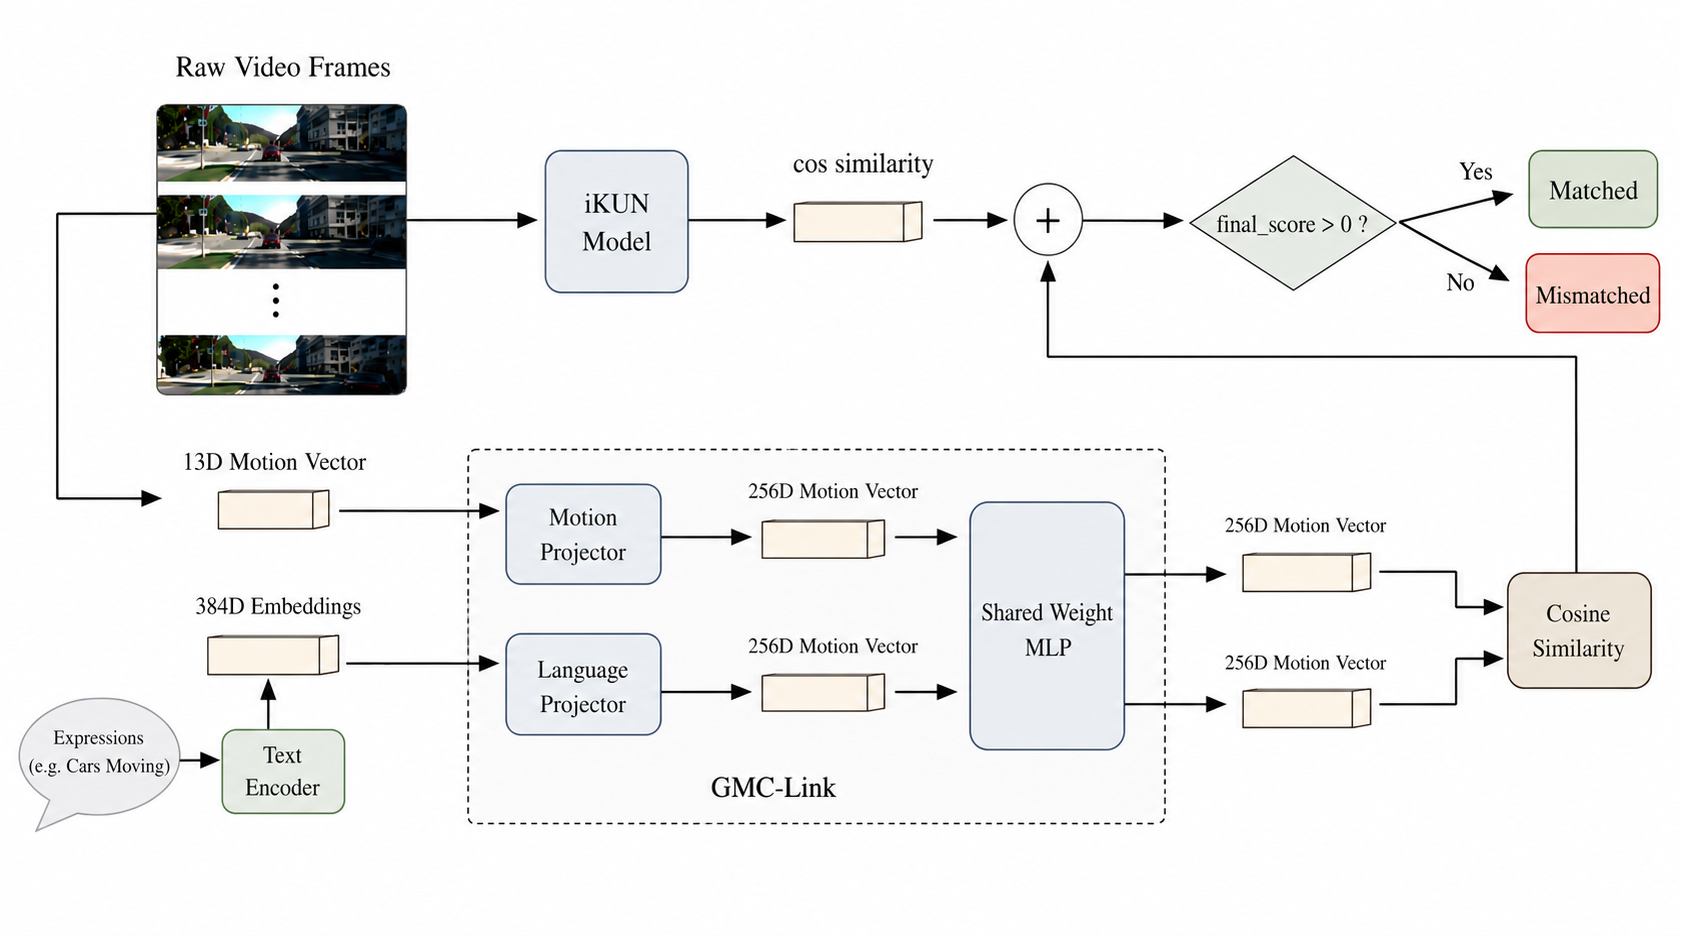
\includegraphics[width=0.82\textwidth]{figures/Architecture.png}
\caption{\textbf{GMC-Link architecture.} The host provides tracks and expression scores; GMC-Link estimates camera motion, derives residual motion, aligns it with language, and returns only a calibrated decision-layer correction.}
\label{fig:architecture}
\end{figure*}

\begin{figure}[t]
\centering
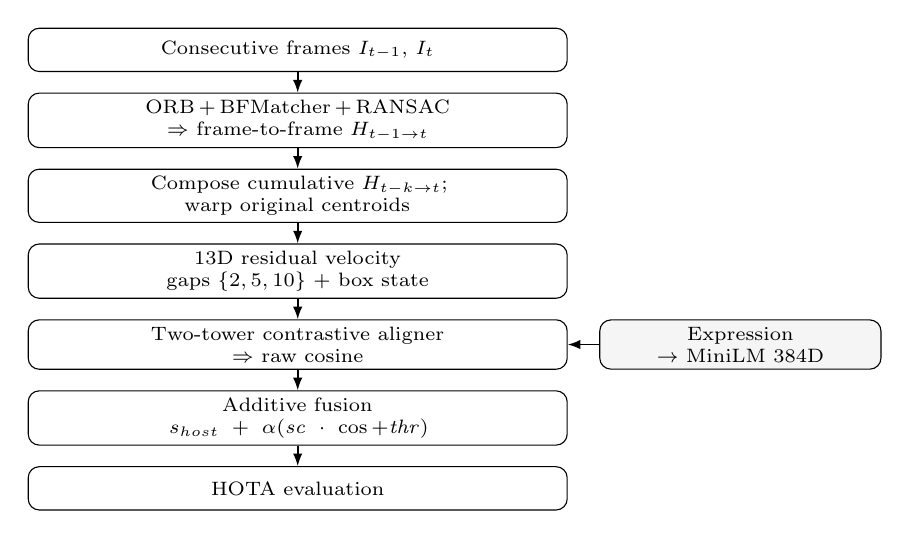
\begin{tikzpicture}[
  font=\scriptsize,
  node distance=2.6mm,
  box/.style={draw, rounded corners, align=center, inner sep=2.5pt,
              text width=0.55\linewidth, minimum height=5.5mm},
  sbox/.style={draw, rounded corners, align=center, inner sep=2.5pt, fill=black!4,
               text width=0.28\linewidth, minimum height=5.5mm},
  ar/.style={-{Latex[length=1.6mm]}, semithick}
]
\node[box] (frames) {Consecutive frames $I_{t-1},\,I_t$};
\node[box, below=of frames] (orb) {ORB\,+\,BFMatcher\,+\,RANSAC\\ $\Rightarrow$ frame-to-frame $H_{t-1\to t}$};
\node[box, below=of orb] (cum) {Compose cumulative $H_{t-k\to t}$;\\ warp original centroids};
\node[box, below=of cum] (desc) {13D residual velocity\\ gaps $\{2,5,10\}$ + box state};
\node[box, below=of desc] (align) {Two-tower contrastive aligner\\ $\Rightarrow$ raw cosine};
\node[box, below=of align] (fuse) {Additive fusion\\ $s_{\text{host}}+\alpha(\mathit{sc}\cdot\cos+\mathit{thr})$};
\node[box, below=of fuse] (hota) {HOTA evaluation};
\node[sbox, right=4mm of align] (text) {Expression\\ $\to$ MiniLM 384D};
\draw[ar] (frames)--(orb);
\draw[ar] (orb)--(cum);
\draw[ar] (cum)--(desc);
\draw[ar] (desc)--(align);
\draw[ar] (align)--(fuse);
\draw[ar] (fuse)--(hota);
\draw[ar] (text)--(align);
\end{tikzpicture}
\caption{\textbf{GMC-Link pipeline.} ORB homographies compose into a cumulative transform, produce a 13D residual-velocity descriptor, align with the expression, and correct the host logit for HOTA evaluation.}
\label{fig:pipeline}
\end{figure}

\subsection{Ego-motion compensation}
\label{sec:ego}

The first stage estimates camera motion between adjacent frames. We detect ORB keypoints~\cite{orb}, match descriptors with a brute-force Hamming matcher, and keep matches passing Lowe's $0.7$ ratio test. Host boxes seed a foreground mask: keypoints inside tracked objects are suppressed so the surviving correspondences are dominated by static background structure rather than moving foreground objects. RANSAC~\cite{ransac} fits $H_{t-1\to t}$ and records median inlier reprojection error as background residual. If too few reliable inliers survive, the stage falls back to identity, so a weak-texture frame degrades to ``no compensation'' rather than to a corrupted camera-motion estimate.

A single homography is exact only for planar or pure-rotation scenes, but driving footage is sufficiently planar-dominated and RANSAC rejects much residual parallax. To reason over a window without repeatedly warping already-warped coordinates, we store the original, never-warped centroids and compose the frame-to-frame transforms into one cumulative homography,
\begin{equation}
H_{t-k\to t} = H_{t-1\to t}\, H_{t-2\to t-1} \cdots H_{t-k\to t-k+1},
\label{eq:cumulative}
\end{equation}
then apply it once to map a past centroid into the current frame, reducing accumulated numerical and interpolation error.

\subsection{Multi-scale residual velocity}
\label{sec:residual}

For temporal gap $g$, raw velocity is centroid displacement and contains both object motion and camera-induced displacement. Ego velocity estimates the displacement caused by the camera alone by warping the past centroid through Eq.~\ref{eq:cumulative}. Residual velocity is their difference,
\begin{equation}
v^{\mathrm{res}}_{g} = v^{\mathrm{raw}}_{g} - v^{\mathrm{ego}}_{g},
\label{eq:residual}
\end{equation}
which approximates the motion a stationary camera would observe. Thus a parked car has near-zero residual motion even as its pixels move significantly under ego-motion. We normalise by image dimensions, $v_{\mathrm{norm}} = (v_{\mathrm{pix}}/d_{\mathrm{img}})\times 100$.

We compute residuals at gaps $\{2,5,10\}$ and concatenate them with box state into a 13D vector ordered as $(\mathit{dx}_s,\mathit{dy}_s)$, $(\mathit{dx}_m,\mathit{dy}_m)$, $(\mathit{dx}_l,\mathit{dy}_l)$, $\Delta w,\Delta h,c_x,c_y,w,h,\mathit{snr}$; the first six entries are residual $(dx,dy)$ pairs at gaps $2$, $5$, and $10$. The scales are complementary rather than redundant: gap $2$ captures short-term jitter, gap $10$ accumulates slow sustained drift, and gap $5$ bridges the two. The final $\mathit{snr}$ is the mid-scale residual object speed relative to the RANSAC-inlier background noise floor. It does not create the class separation itself, but represents homography reliability and reduces frame-level score variance when compensation is weak.

\subsection{Motion-language alignment}
\label{sec:align}

A two-tower encoder maps the 13D motion vector and expression into a shared space. Linear adapters (motion $13\!\to\!256$, language $384\!\to\!256$ from all-MiniLM-L6-v2~\cite{sbert}) feed a shared MLP ($256\!\to\!512\!\to\!512\!\to\!256$), layer norm, and $\ell_2$ normalisation. Training uses symmetric InfoNCE~\cite{infonce} at temperature $0.07$ with shared-expression false negatives masked. Inference uses raw cosine similarity, with no sigmoid or temporal smoothing, so the fusion layer receives an uncalibrated alignment score. CLIP-text lifted pooled HOTA on one host but regressed within-class scores under the shipped raw-cosine pipeline, and larger 768D sentence encoders were flat to negative, so MiniLM stays. The aligner is intentionally standard; the paper's design budget is spent on ego-motion compensation and decision-level calibration.

\subsection{Decision-level additive fusion}
\label{sec:fusion}

The alignment score corrects the host logit at the decision level. We inject it additively per host and per axis,
\begin{equation}
s_{\mathrm{final}} = s_{\mathrm{model}} + \alpha\,\bigl(\mathit{sc}\cdot\cos + \mathit{thr}\bigr),
\label{eq:fusion}
\end{equation}
where $\cos$ is raw motion-language cosine, $\mathit{sc}$ rescales it to the host logit range, $\mathit{thr}$ shifts the operating point, and $\alpha$ sets weight. We use decision-level fusion because feature-level motion injection into the visual encoder regressed an early pipeline by $-21.7\%$ F1; the correction is applied only after the host has formed its appearance representation. This also keeps the module auditable: the host score and motion correction remain separate terms, so a failure can be traced to appearance grounding, ego-motion estimation, motion-language alignment, or calibration.

A keyword router selects the motion recipe when an expression contains one of $15$ fixed motion substrings (e.g.\ \emph{moving}, \emph{turning}, \emph{parked}, \emph{braking}); otherwise it selects the appearance recipe. Because motion evidence is largely uninformative for appearance-only expressions, $\mathit{sc}_{\mathrm{appear}}$ is seven to eleven times smaller than $\mathit{sc}_{\mathrm{motion}}$. The coefficients absorb host-specific logit-scale differences, so the table should be read as calibration to each host's score range rather than as a learned fusion head.

\begin{table}[t]
\centering
\caption{Locked fusion coefficients for Eq.~\ref{eq:fusion}. Appearance scale is damped because motion is uninformative on appearance expressions.}
\label{tab:recipe}
\small
\begin{tabular}{llccc}
\toprule
Host & Axis & $\alpha$ & $\mathit{sc}$ & $\mathit{thr}$ \\
\midrule
\multirow{2}{*}{iKUN}        & motion     & 1.00 & 0.90 & $+0.17$ \\
                             & appearance & 1.00 & 0.30 & $+0.10$ \\
\midrule
\multirow{2}{*}{FlexHook (V1)} & motion     & 0.65 & 10.0 & $+3.0$  \\
                             & appearance & 1.00 & 3.50 & $+0.9$  \\
\midrule
\multirow{2}{*}{FlexHook (V2)} & motion     & 0.40 & 10.0 & $+1.3$  \\
                             & appearance & 1.00 & 3.50 & $+1.2$  \\
\bottomrule
\end{tabular}
\end{table}

Standard-deviation matching and a learned fusion network were tested but underperformed this fixed scalar calibration.

\section{Experiments}
\label{sec:exp}

\subsection{Setup}
\label{sec:setup}

We evaluate on Refer-KITTI V1~\cite{transrmot} (3-sequence pooled test) and V2~\cite{temprmot} (4-sequence pooled test), using TrackEval HOTA~\cite{hota}. The public V1 convention reports a canonical iKUN score of $44.564$, so we keep that paper anchor. We study iKUN~\cite{ikun} and FlexHook~\cite{flexhook} in three host--split settings; FlexHook (V1/V2) is one architecture calibrated per split, not two independent methods. Results are mean$\pm$std over $n{=}3$ seeds for cross-setting tables and $n{=}5$ for ablations with Welch tests. The aligner uses AdamW ($10^{-3}$, batch $256$, $100$ epochs); ORB uses $1500$ features and RANSAC a $5$\,px threshold. We report native hosts and a simple uncalibrated raw-cosine GMC control to separate adding the signal from calibrating it to the host logit scale. Refer-KITTI has no held-out tuning split, so Table~\ref{tab:recipe}'s shipped coefficients are calibrated on the benchmark sequences and should not be claimed as universally transferable hyperparameters. Because these coefficients are benchmark calibration rather than transferable hyperparameters, we use leave-one-sequence-out calibration to bound overfitting risk. iKUN LOSO moving HOTA remains $28.38 \pm 1.60$ versus $29.47 \pm 0.88$ in-sample (native $20.25$), while FlexHook LOSO pooled is $53.28 \pm 0.17$ (V1) and $42.74 \pm 0.07$ (V2), with V2 still above the published $42.526$. We therefore claim the iKUN moving-class recovery and the FlexHook V2 pooled gain, not the iKUN pooled number, as the calibration-robust results.

The test splits are heavily skewed toward appearance. V1 holds $158$ expressions over $1010$ frames, of which $75.3\%$ are appearance queries, $7.6\%$ are static-motion queries, and only $17.1\%$ ($27$ expressions) refer to a moving object; V2 holds $862$ expressions over $1469$ frames with a similar $74.1\,/\,11.7\,/\,14.2$ split. The motion class our module targets is therefore a roughly one-in-six minority. Pooled HOTA is computed once over the union of all trajectories, so it is dominated by detection and association counts from the appearance majority; it is not a class-weighted mean of per-class HOTA. A recovery concentrated on moving expressions can therefore register as a small pooled movement even when the per-class effect is large. We treat moving-class HOTA as the primary diagnostic and report pooled HOTA as the whole-benchmark check.

\subsection{Main results}
\label{sec:main}

Table~\ref{tab:main} reports pooled HOTA. On iKUN~\cite{ikun}, GMC-Link reaches $44.634 \pm 0.066$, matching rather than materially beating the published $44.564$. The uncalibrated control is negative on iKUN and FlexHook V1, showing that raw cosine contains useful evidence but must be scaled to the host logit. The gain appears where expected: iKUN has the weakest native motion score and the largest moving-class gain ($+8.83$, Table~\ref{tab:deficit}). FlexHook V2 gives the clean pooled improvement, $42.807 \pm 0.038$ versus published $42.526$ ($+0.281$). FlexHook V1 improves over \emph{+GMC simple} ($53.121 \to 53.526$) but remains below its published $53.824$.\footnote{No tested configuration beats FlexHook V1's published $53.824$; the strongest legacy variant reaches $53.716 \pm 0.068$ ($n{=}3$), so we report the gain against \emph{+GMC simple}.} We compare each host to its own native score because stronger motion-language hosts such as VMRMOT~\cite{vmrmot} use different detectors and trackers.

\begin{table}[t]
\centering
\caption{Pooled HOTA on Refer-KITTI test ($n{=}3$, mean$\pm$std). $\Delta$ is against published pooled HOTA; iKUN matches, while FlexHook V2 is the clean pooled improvement.}
\label{tab:main}
\small
\setlength{\tabcolsep}{4pt}
\begin{tabular}{lcccc}
\toprule
Host & Native & +GMC simple & +GMC (ship) & $\Delta$ paper \\
\midrule
iKUN~\cite{ikun} (V1)        & 44.564 & 44.272 & $44.634 \pm 0.066$ & $+0.070$ \\
FlexHook (V1)~\cite{flexhook}  & 53.824 & 53.121 & $53.526 \pm 0.087$ & $-0.298$\textsuperscript{$\dagger$} \\
FlexHook (V2)~\cite{flexhook}  & 42.526 & 42.532 & $42.807 \pm 0.038$ & $+0.281$ \\
\bottomrule
\end{tabular}
\\[2pt]
{\footnotesize \textsuperscript{$\dagger$}FlexHook (V1) paper gap is structural (no tested configuration beats $53.824$); $\Delta$ vs \emph{+GMC simple} anchor $= +0.405$.}
\end{table}

\subsection{The motion deficit}
\label{sec:deficit}

The gain tracks native motion deficit. iKUN starts lowest and gains most ($+8.83 \pm 0.83$); FlexHook V1 and V2 start higher and gain little ($+0.91 \pm 0.79$ and $+0.43 \pm 0.17$). Across the three settings, the relation is monotone-inverse: larger native deficit receives larger correction. This is the main claim of the paper, not the small pooled iKUN delta. It says the module is most useful when the host already grounds appearance but does not reliably distinguish ego-induced displacement from object motion. We treat the pattern as a prediction over three settings, not a proportional law.

\begin{table}[t]
\centering
\caption{Motion deficit across host--split settings. Native moving-class HOTA versus the moving-class HOTA gain added by the module. The gain is monotone-inverse to native motion ability across the three settings.}
\label{tab:deficit}
\small
\begin{tabular}{lcc}
\toprule
Host & Native MOVING & GMC MOVING gain \\
\midrule
iKUN~\cite{ikun}             & 20.25 & $+8.83 \pm 0.83$ ($n{=}5$) \\
FlexHook (V1)~\cite{flexhook}  & 43.98 & $+0.91 \pm 0.79$ ($n{=}3$) \\
FlexHook (V2)~\cite{flexhook}  & 48.02 & $+0.43 \pm 0.17$ ($n{=}3$) \\
\bottomrule
\end{tabular}
\end{table}

\subsection{Ablations}
\label{sec:ablation}

Table~\ref{tab:ablation} strips one component at a time on iKUN moving-class HOTA. The full module lifts $20.25\to29.08$ ($+8.83$). Among engineered components, only ego-compensation is significant: raw velocity costs $-1.77$ (Welch $t{=}3.75$, $p{=}0.006$). Single-gap motion ($-0.26$, $p{=}0.64$) and removing snr ($+0.67$, $p{=}0.19$) fall within seed spread.

\begin{table}[t]
\centering
\caption{Moving-class HOTA ablation on iKUN ($n{=}5$). Ego-compensation is the only significant engineered component ($-1.77$, Welch $p{=}0.006$).}
\label{tab:ablation}
\small
\begin{tabular}{lc}
\toprule
Variant & MOVING HOTA \\
\midrule
Native host (no module)           & 20.25 \\
Full module                       & \textbf{29.08 $\pm$ 0.83} \\
\;\;$-$ego (raw velocity)         & 27.31 $\pm$ 0.66 \\
\;\;$-$multiscale (single gap)    & 28.82 $\pm$ 0.84 \\
\;\;$-$snr                        & 29.74 $\pm$ 0.59 \\
\bottomrule
\end{tabular}
\end{table}

Feature-level injection regressed an early host by $-21.7\%$ F1, so the module corrects logits after appearance scoring rather than reshaping host representations.

\begin{figure}[t]
\centering
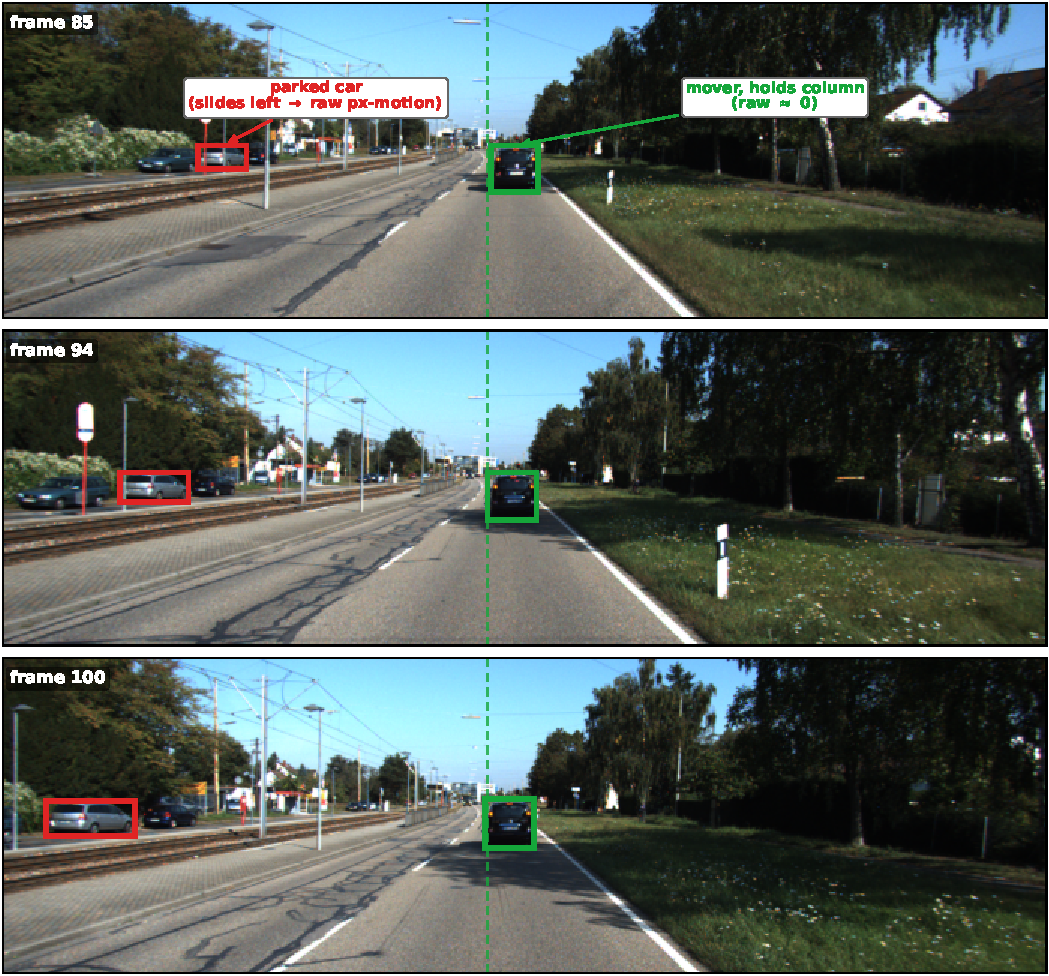
\includegraphics[width=\linewidth]{figures/qualitative.pdf}
\caption{\textbf{Real recovery under camera ego-motion} on ``moving cars'' (Refer-KITTI seq 0005, frames 85/94/100 of a forward-driving clip; the green car moves, the red car is parked). The dashed line marks the mover's image column. \textbf{Red:} the parked car's centroid slides left as the camera passes it (center-$x$ $261\!\to\!104$\,px), so the camera-naive host scores it ``moving'' (false positive), yet its ego-compensated residual is near zero and the module restores it to static. \textbf{Green:} the moving car holds its column (center-$x$ ${\approx}605$, ${<}1$\,px/frame), so the host misses it (false negative), but its nonzero residual --- unlike the static background --- recovers it as moving. Both errors flip from the same host logit through the additive correction.}
\label{fig:qual}
\end{figure}

The module runs at $68$ FPS (median $14.8$\,ms/frame excluding host inference), dominated by CPU ORB homography ($14.55$\,ms); the aligner is under $0.2$\,ms. This is $6.7\times$ the benchmark's $10$ fps capture rate.\footnote{An orthogonal appearance re-ranker reaches $45.612$ pooled HOTA on iKUN ($n{=}3$); we do not claim it here.}

\section{Conclusion and Limitations}
\label{sec:conclusion}
A decision-level ego-motion module recovers motion-class referring expressions that camera-naive hosts miss. The recovered signal grows as native motion ability shrinks: across the three host--split settings studied, the gain is monotone-inverse to native motion ability. The module keeps the tracker and detector fixed, retrains no host weights, and adds only per-setting scalar calibration. On iKUN~\cite{ikun} it matches published pooled HOTA while lifting the hidden motion class; on FlexHook~\cite{flexhook} V2 it improves pooled HOTA outright.

The limits are bounded. A single ORB/RANSAC homography~\cite{botsort} is exact only for planar or pure-rotation scenes. Our evidence is therefore confined to planar-dominated Refer-KITTI driving footage, with no claim of transfer to handheld, aerial, or strongly non-planar video. Foreground masks come from host boxes; bad detections can leak object features into the ego estimate, although RANSAC and identity fallback bound the failure. We evaluate only two-stage referring-by-tracking hosts; end-to-end hosts expose analogous scores but are untested. Hosts with native temporal memory, such as TempRMOT~\cite{temprmot}, are out of scope because they already aggregate trajectory history.

The open lever is a stronger motion representation: the alignment ceiling sits in the descriptor, not the fusion stage, so richer features encoding the trajectory geometry a 2D vector flattens are the natural next step for the TransRMOT~\cite{transrmot} lineage of camera-naive hosts.

\bibliographystyle{ACM-Reference-Format}
\bibliography{refs}

\end{document}
